
\section{Hybrid positioning}

The absolute positioning method is quit accurate but still it suffers from noise. On the other hand relative position has a lot uncertainty, because of the physical interference. By combing these two positioning methods we can get more precise location based on sensor measurements from absolute and prediction from the relative positions. This combination is called hybrid positioning. One of the methods achieving hybrid position is with Kalman filter, which will be described below.

\subsection{Kalman filter}

The Kalman filter was made by Rudolf E. Kalman. It was developed for Apollo mission to the moon, to track the location of the space shuttle. This method is still used, because it dos not require a lot of processing power and memory space. The reasoning is that the method dos not need to save any data apart the model of movement and and previews position. The process of filter is predict using model and previous position. After the prediction the measurement are coming and the filter is multiplying both Gaussian distribution. By multiplying the filter is correcting its estimation and making more precise location.

	\begin{figure}[H]
	\centering
	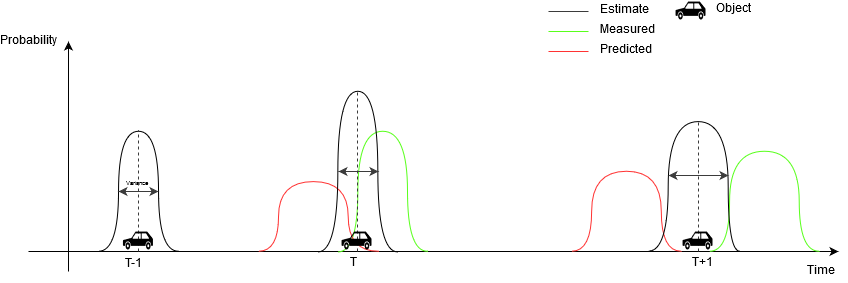
\includegraphics[width=0.7\linewidth]{positioning/positioning/DiagramKalman}
	\caption{Kalmans filter principal}
	\label{fig:Kalmanfilter}
	\end{figure}

In the Figure\ref{fig:Kalmanfilter} we can see basic principal of how the filter is working there are two cases in it. First one is when time is (T-1) and time is (T). In this case we can see that the filter goes closer to the measurement Gaussian, because it is more reliable. Also from the graph we can see the power of hybrid position, the probability is higher then absolute and relative positioning. The second case is in the period (T) and (T+1) in this case the measurements has a lot more noise in them. Then the estimation is moving further from the measurement Gaussian, because of the lower probability. 